\section{Einführung}

\begin{frame}
	\frametitle{ILP}

	\begin{block}{Was ist ILP}
		\begin{itemize}
			\item Die Schnittstelle zwischen Machine Learning und logischer Programmierung
			\item {Idee: Formalisierung der \textit{Umgebung}
				\begin{itemize}
					\item Basis: Background-Knowledge, positive und negative Beispiele
					\item Darstellung in Form von Klauseln
					\item Generierung neues Wissens durch finden von Hypothesen die positive
					Klauseln erfüllen, negative nicht.
				\end{itemize}
			}
		\end{itemize}
	\end{block}
	Wieso induktiv?
	$\Rightarrow$ Lösen von Problemen vom spezifischen zum generellen
\end{frame}

\subsection{First order logic}
\begin{frame}
	\frametitle{FOL}
	\begin{block}{}
	In FOL besteht die Welt aus
	% TODO: Begriffe nochmal genauer anschauen: Insbesondere Atome
	\begin{itemize}
		\item Objekten   (Personen, Dingen)
		\item Relationen $(>, <)$
		\item Funktionen $(+, -)$
	\end{itemize}
	\end{block}

	Terme beschreiben Objekte in der Welt:
	\begin{itemize}
		\item Konstanten ($2$, Chuck Norris, \ldots)
		\item Variablen (x,y, a, \ldots)
		\item Funktionen $(Term_1, \ldots, Term_n)$
	\end{itemize}
	\textit{Ground term}: Term ohne Variablen


	\begin{block}{}
		Atome/Literale sind kleinstmögliche Ausdrücke, die wahr/falsch sind
		\begin{itemize}
			\item $predicate(Term_1, \ldots, Term_n)$\\ 
				father(bob)
			\item $Term_1 = Term_2 \Leftarrow$ Gleicheitsrelation
		\end{itemize}
	\end{block}

\end{frame}

\begin{frame}
	\frametitle{FOL}
	Horn Clauses:

	\begin{align*}
		\neg C_1 \vee \neg C_2 \vee \ldots \vee \neg C_n  \vee C_{n+1} \Leftrightarrow\\
		C_1 \wedge C_2 \wedge \ldots \wedge C_n  \rightarrow C_{n+1}
	\end{align*}

	ILP verwendet zumeist \textit{definite program clauses} vom Typ:

	\begin{align*}
		\underbrace{T}_{\text{head}} \Leftarrow \underbrace{L_1, \ldots, L_m}_{\text{body}}
	\end{align*}
	wobei $T, L_1, \ldots, L_m$ Atome sind und nur $T$ positiv ist.

	Beispiel:
	\begin{align*}
		daughter(X,Y) \Leftarrow female(X), mother(Y, X)
	\end{align*}
\end{frame}

\begin{frame}
	\frametitle{Art der Logik -- Beispiel}

	\begin{block}{Pokerspiel}
	Konstanten: $Rank = \{7,8,9,10,j,q,k,a\}$\\
	            $Suit = \{hearts, spaces, club, diamonds\}$
	
	Beschreibung von Karo 7 als Horn Clause: $card(diamonds, 7)$

	$card$: Prädikat\\
	$diamonds, 7$: Konstanten

	Definieren von Paaren:\\
	$\underbrace{pair(}_{\text{Prädikat}}\underbrace{card}_{\text{Funktion}}(diamonds, 7),
	card(hearts, 7))$

	Allgemein:\\
	$pair(card(Suit_1, Rank_1),card(Suit_2, Rank_2)) \Leftarrow \underbrace{Rank_1 =
	Rank_2}_{(Rank_1=7 \wedge Rank_2=7) \vee \ldots}$

	\end{block}
	
\end{frame}

\begin{frame}
\frametitle{Hypothesen, Beispiele etc}
	\emph{Gegeben:} Background-Knowledge $(B)$, Menge von positiven $(E^+)$ und negativen $(E^-)$ Beispielen\\
	\emph{Ziel:} Finden einer Hypothese $(\mathcal{H})$ die alle positiven und kein negatives Beispiele erfüllt
\begin{figure}[H]
	\centering
	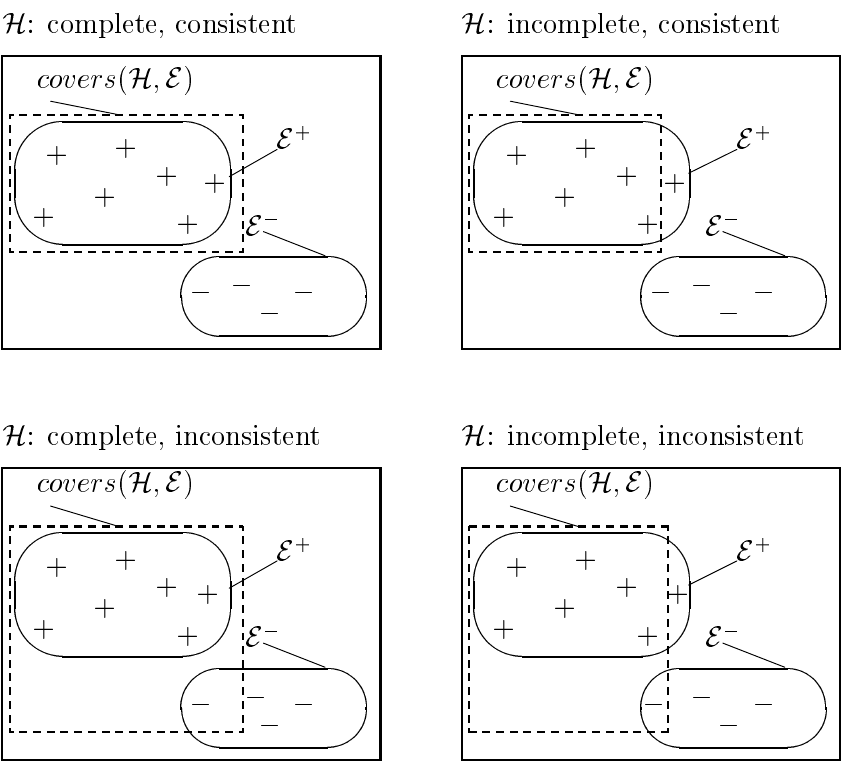
\includegraphics[width=0.5\textwidth]{hypothesis}
\end{figure}
\end{frame}
